\documentclass[12pt]{article}
\usepackage[utf8]{inputenc}
\usepackage{amsmath, amssymb,multicol}
\usepackage{hyperref}
\usepackage{tikz}
\usepackage[left=2.5cm,right=2.5cm,bottom=2.5cm]{geometry}
\usetikzlibrary{arrows, arrows.meta, positioning, bending, quotes}
\hypersetup{
    colorlinks=true}

\title{MATH 5707 (Spring 2026): Homework 8}
\date{}

\begin{document}
\vspace{-0.7in}

\maketitle
\vspace{-0.6in}


\section*{Directions and Introduction}
Submit a pdf of your solutions to the HW 8 assignment on Gradescope by 11:59 pm on April 10.

Problem 2 is marked as a peer review problem. \href{https://docs.google.com/document/d/1jSw9pmMJJFUx_6dTkcUi4k4HJNIrrIIgs9zdWhAycx0/edit?usp=sharing}{This document gives directions and deadlines for the peer review process.}



\section*{Problems}

\begin{enumerate}
\item[0.] If you would like any of these problems to be graded for proficiency with the key skills, list the skill and the corresponding problem.  If you want to label the skill by number, use the numbering that is in the syllabus.
  \item Draw the block-cut-vertex tree for the following graph. \\
  \begin{center}
  
  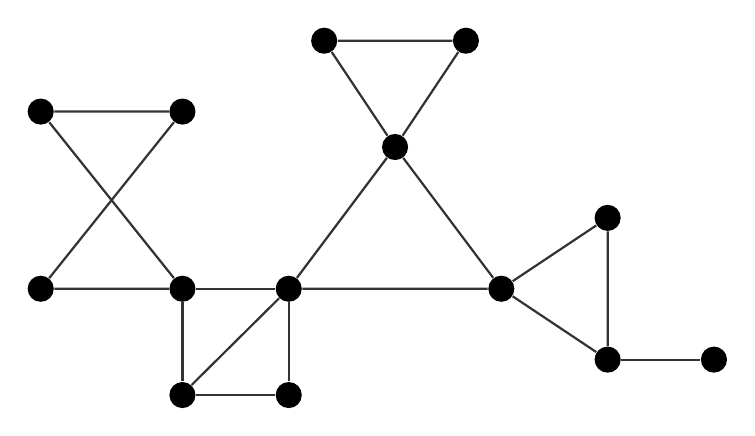
\begin{tikzpicture}[
    scale=0.9,
    % Styles for original graph
    edge/.style={thick, draw=black!80}
]

        
        % --- Cut Vertices ---
        \node[fill,circle] (c1) at (0, 1.5) {};
        \node[fill,circle] (c2) at (-1.5, -0.5) {};
        \node[fill,circle] (c3) at (1.5, -0.5) {};
        \node[fill,circle] (c4) at (3, -1.5) {};
        \node[fill,circle] (c5) at (-3, -0.5) {};
        

        % --- Normal Vertices ---
        % Vertices for Block 2 (Top Triangle)
        \node[fill,circle] (t1) at (-1, 3.0) {};
        \node[fill,circle] (t2) at (1, 3.0) {};
        
        % Vertices for Block 3 (Left Square)
        \node[fill,circle] (l2) at (-3, -2.0) {};
        \node[fill,circle] (l3) at (-1.5, -2.0) {};
        
        % Vertex for Block 4 (Right Triangle)
        \node[fill,circle] (r1) at (3, 0.5) {};
        
        % Vertex for Block 5 (Far Right Bridge)
        \node[fill,circle] (e1) at (4.5, -1.5) {};

 % Vertices for Block  6 (far Left Square)
        \node[fill,circle] (fl1) at (-5, -0.5) {};
        \node[fill,circle] (fl2) at (-5, 2.0) {};
        \node[fill,circle] (fl3) at (-3, 2.0) {};

        % --- Edges ---
        % Block 1: Central Triangle
        \draw[edge] (c1) -- (c2) -- (c3) -- (c1); 
        % Block 2: Top Triangle
        \draw[edge] (c1) -- (t1) -- (t2) -- (c1); 
        % Block 3: Left Square
        \draw[edge] (c2) -- (c5) -- (l2) -- (l3) -- (c2); 
        \draw[edge] (c2)--(l2);
        % Block 4: Right Triangle
        \draw[edge] (c3) -- (r1) -- (c4) -- (c3); 
        % Block 5: Bridge / Edge
        \draw[edge] (c4) -- (e1); 
        %Block 6: square
        
      \draw[edge] (fl1) -- (c5) -- (fl2) -- (fl3) -- (fl1); 

    \end{tikzpicture}
    \end{center}
    \item(Peer review problem; Each part is worth 4 points and
graded as a separate problem.) Draw a graph $G$ that satisfies the following properties, or explain why no such graph can exist.

\begin{enumerate}
\item A $3$-edge connected graph with some set of $3$ edges $E'$ such that $G-E'$ has at least 3 connected components.  
\item A $3$-vertex connected graph with some set of $3$ vertices $V'$ such that $G-V'$ has at least $3$ connected components. 
\end{enumerate}
   
   \item (Bondy-Murty 11.1.1) For each of the following digraphs, determine all possible $x,y$-flows and the value of a maximum flow. 
   \begin{multicols}{2}
   \begin{enumerate}
   \item \begin{center}
    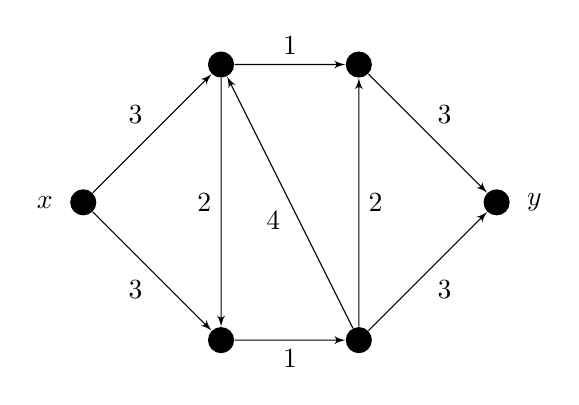
\begin{tikzpicture}[scale=1.75]

\tikzset{vertex/.style = {shape=circle,fill,minimum size=0.5em}}
\tikzset{every path/.style = {->,> = latex'}}
% vertices
\node[vertex] (a) at  (0,0) {};
\node[left=0.75em] at (0,0) {$x$};
\node[vertex] (b) at  (1,-1) {};
\node[vertex] (c) at  (2,-1) {};
\node[vertex] (d) at  (3,0) {};
\node[right=0.75em] at (3,0) {$y$};
\node[vertex] (e) at  (1,1) {};
\node[vertex] (f) at  (2,1) {};
%edges
\path (a) edge["$3$",swap] (b);
\path (b) edge["$1$",swap] (c);
\path (c) edge["$3$", swap] (d);
\path (a) edge["$3$"] (e);
\path (e) edge["$1$"] (f);
\path (f) edge["$3$"] (d);
\path (e) edge["$2$", swap] (b);
\path (c) edge["$4$"] (e);
\path (c) edge["$2$",swap] (f);
\end{tikzpicture}
\end{center}
\item  \begin{center}
    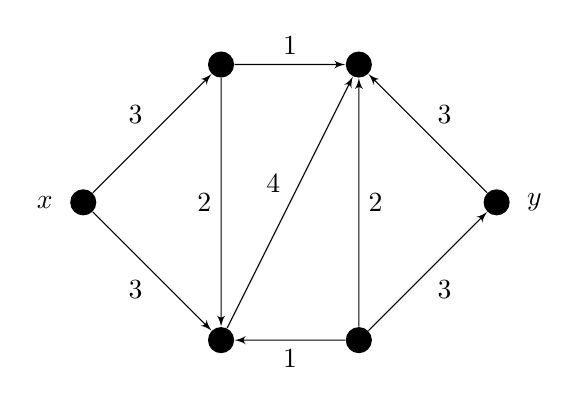
\begin{tikzpicture}[scale=1.75]

\tikzset{vertex/.style = {shape=circle,fill,minimum size=0.5em}}
\tikzset{every path/.style = {->,> = latex'}}
% vertices
\node[vertex] (a) at  (0,0) {};
\node[left=0.75em] at (0,0) {$x$};
\node[vertex] (b) at  (1,-1) {};
\node[vertex] (c) at  (2,-1) {};
\node[vertex] (d) at  (3,0) {};
\node[right=0.75em] at (3,0) {$y$};
\node[vertex] (e) at  (1,1) {};
\node[vertex] (f) at  (2,1) {};
%edges
\path (a) edge["$3$",swap] (b);
\path (c) edge["$1$"] (b);
\path (c) edge["$3$",swap] (d);
\path (a) edge["$3$"] (e);
\path (e) edge["$1$"] (f);
\path (d) edge["$3$",swap] (f);
\path (e) edge["$2$", swap] (b);
\path (b) edge["$4$"] (f);
\path (c) edge["$2$",swap] (f);
\end{tikzpicture}
\end{center}

   \end{enumerate}
     \end{multicols}
    \item (Bondy-Murty 11.2.1) In the following network (the capacities are labeled in the left picture and the flows are labeled in the right picture):
    \begin{enumerate}
    \item Determine all $x,y$-cuts. 
    \item Find the capacity of the minimum cut.
    \item Show that the flow indicated (in the graph on the right) is a maximum flow. 
    \end{enumerate}
    \begin{center}
    
    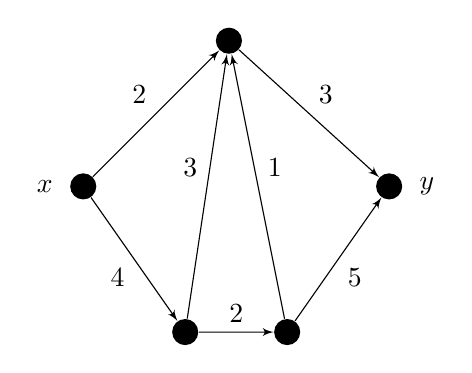
\begin{tikzpicture}[scale=1.85]

\tikzset{vertex/.style = {shape=circle,fill,minimum size=0.5em}}
\tikzset{every path/.style = {->,> = latex'}}
% vertices
\node[vertex] (a) at  (0,0) {};
\node[left=0.75em] at (0,0) {$x$};
\node[vertex] (b) at  (0.7,-1) {};
\node[vertex] (c) at  (1.4,-1) {};
\node[vertex] (d) at  (2.1,0) {};
\node[right=0.75em] at (2.1,0) {$y$};
\node[vertex] (e) at  (1,1) {};
%edges
\path (a) edge["$4$",swap] (b);
\path (b) edge["$2$"] (c);
\path (c) edge["$5$",swap] (d);
\path (a) edge["$2$"] (e);
\path (e) edge["$3$"] (d);
\path (b) edge["$3$"] (e);
\path (c) edge["$1$", swap] (e);
\end{tikzpicture}$\qquad$
    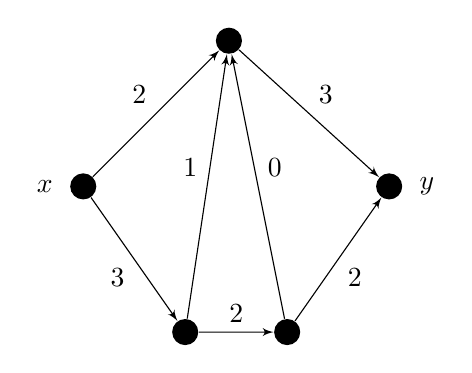
\begin{tikzpicture}[scale=1.85]
\tikzset{vertex/.style = {shape=circle,fill,minimum size=0.5em}}
\tikzset{every path/.style = {->,> = latex'}}
% vertices
\node[vertex] (a) at  (0,0) {};
\node[left=0.75em] at (0,0) {$x$};
\node[vertex] (b) at  (0.7,-1) {};
\node[vertex] (c) at  (1.4,-1) {};
\node[vertex] (d) at  (2.1,0) {};
\node[right=0.75em] at (2.1,0) {$y$};
\node[vertex] (e) at  (1,1) {};
%edges
\path (a) edge["$3$",swap] (b);
\path (b) edge["$2$"] (c);
\path (c) edge["$2$",swap] (d);
\path (a) edge["$2$"] (e);
\path (e) edge["$3$"] (d);
\path (b) edge["$1$"] (e);
\path (c) edge["$0$", swap] (e);
\end{tikzpicture}
\end{center}
    
  
\end{enumerate}

\end{document}